%%\documentclass[a4paper, 12pt]{scrreprt}

\documentclass[a4paper, 12pt]{scrartcl}
%usepackage[german]{babel}
\usepackage{microtype}
%\usepackage{amsmath}
%usepackage{color}
\usepackage[utf8]{inputenc}
\usepackage[T1]{fontenc}
\usepackage{wrapfig}
\usepackage{lipsum}% Dummy-Text
\usepackage{multicol}
\usepackage{alltt}
%%%%%%%%%%%%bis hierhin alle nötigen userpackage
\usepackage{tabularx}
\usepackage[utf8]{inputenc}
\usepackage{amsmath}
\usepackage{amsfonts}
\usepackage{amssymb}

%\usepackage{wrapfig}
\usepackage[ngerman]{babel}
\usepackage[left=25mm,top=25mm,right=25mm,bottom=25mm]{geometry}
%\usepackage{floatrow}
\setlength{\parindent}{0em}
\usepackage[font=footnotesize,labelfont=bf]{caption}
\numberwithin{figure}{section}
\numberwithin{table}{section}
\usepackage{subcaption}
\usepackage{float}
\usepackage{url}
%\usepackage{fancyhdr}
\usepackage{array}
\usepackage{geometry}
%\usepackage[nottoc,numbib]{tocbibind}
\usepackage[pdfpagelabels=true]{hyperref}
\usepackage[font=footnotesize,labelfont=bf]{caption}
\usepackage[T1]{fontenc}
\usepackage {palatino}
%\usepackage[numbers,super]{natbib}
%\usepackage{textcomp}
\usepackage[version=4]{mhchem}
\usepackage{subcaption}
\captionsetup{format=plain}
\usepackage[nomessages]{fp}
\usepackage{siunitx}
\sisetup{exponent-product = \cdot, output-product = \cdot}
\usepackage{hyperref}
\usepackage{longtable}
\newcolumntype{L}[1]{>{\raggedright\arraybackslash}p{#1}} % linksbündig mit Breitenangabe
\newcolumntype{C}[1]{>{\centering\arraybackslash}p{#1}} % zentriert mit Breitenangabe
\newcolumntype{R}[1]{>{\raggedleft\arraybackslash}p{#1}} % rechtsbündig mit Breitenangabe
\usepackage{booktabs}
\renewcommand*{\doublerulesep}{1ex}
\usepackage{graphicx}
\usepackage{chemformula}


\usepackage[backend=bibtex, style=chem-angew, backref=none, backrefstyle=all+]{biblatex}
\bibliography{Literatur.bib}
\defbibheading{head}{\section{Literatur}\label{sec:Lit}} 
\let\cite=\supercite
%\begin{document}
\section{Durchführung}
Zur Charakterisierung verschiedenen Laser unbekannter Wellenlänge wurde dessen Beugungsverhalten an einem Spalt untersucht. Hierfür wurde zuerst ein Strahlengang mit einem Laser bekannter Wellenlänge als Lichtquelle aufgebaut um eine Referenzierung zu erhalten. Der lineare Strahlengang wird im folgenden ausgehend vom Detektor bis hin zur Lichtquelle beschrieben. Der Detektor, in der Form einer Monochrom-Kamera mit einem CMOS-Chip, wurde in direkter Verbindung mit dem Messrechner aufgebaut. Die empfindlichen Fläche wurde als 4,512 mm × 2,880 mm groß gegeben und durch eine Einbuchtung in dem Kameragehäuse kenntlich gemacht. Der Detektor wurde in $11.9 \,[\si{cm}]$ Entfernung zur Sammellinse im Strahlengang aufgestellt, entsprechend der zuvor empirisch bestimmten Brennweite der verwendeten Sammellinse. Demzufolge konnte der Brennpunkt der Linse leicht in den Detektor ausgerichtet werden. In $10 \,[\si{cm}]$ Entfernung zur Linse wurde der verwendete justierbarer Einzelspalt aufgestellt, welcher orthogonal zur Tischebene ausgerichtet und justiert wurde. Des weiteren ist ein Polarisationsfilter benutzt worden um die Lichtintensität abzuschwächen, damit das Sättigungsniveau des Detektors nicht erreicht wird, und eine klare Intensitätsmessung durchgeführt werden konnte. Dieser sowie die Lichtquelle in Form des jeweiligen Lasers wurden frei im Strahlengang, ungefähr in zwanzig und dreißig Zentimeter Entfernung zum Spalt, aufgestellt. Nach erfolgreicher Ausrichtung des Lasers durch die Bauelemente des Strahlengangs in den Detektor wurden für den Referenzlaser, als Helium-Neon der Laserklasse II, drei Messungen des Beugungsbildes durchgeführt. Von besonderer Relevanz bei der Ausrichtung war die orthogonale Lage des Lasers zum Beugungsspaltes, welche durch drehen des runden Lasergehäuses in seiner Fassung erreicht wurde. Für die folgenden drei zu charakterisierenden Laser wurde jeweils eine Messung durchgeführt. Der schematische Versuchsaufbau ist der folgenden Abbildung zu entnehmen. 
\\
\begin{figure}[H]
	\centering	
	\begin{minipage}{1\textwidth}
		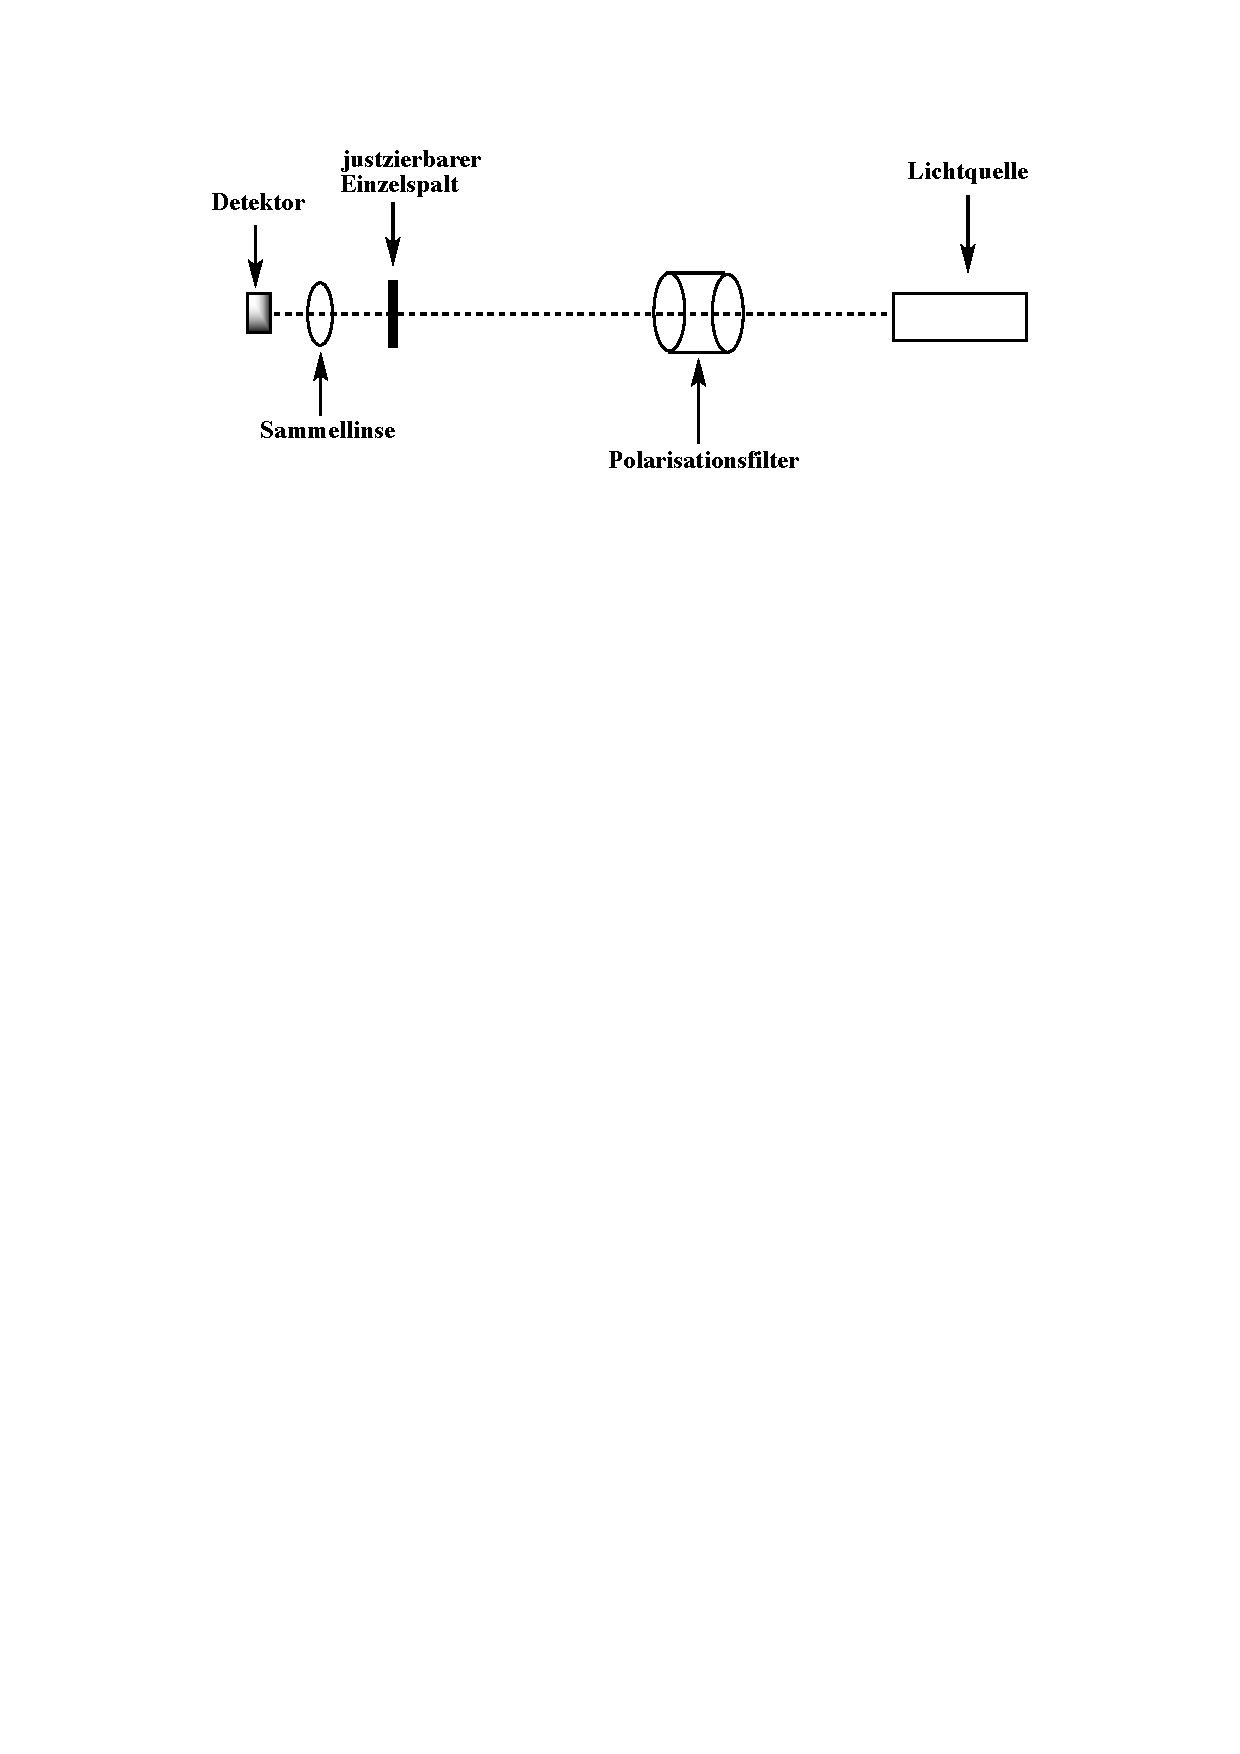
\includegraphics[width=\columnwidth]{Bilder/Versuchsaufbau.pdf}
	\end{minipage}
	\caption{Schematischer Aufbau des durchgeführten Versuchs.}
	\label{Versuchsaufbau}
\end{figure} 
%\end{document}
